%scrrprt ist eine Klasse für Berichte und längere Arbeiten
\documentclass[11pt,a4paper]{scrreprt}
%ermöglicht die Eingabe von Umlauten usw. ohne Codierung
\usepackage[utf8]{inputenc}
%Schriften werden mit einer passenden Kodierung für europäische Zeichen ausgegeben
\usepackage[T1]{fontenc}
%Passt Dokumentelemente an die Konventionen der deutschen Sprache (neue Rechtschreibung) an, z.b. Datumsangaben, Silbentrennung
\usepackage[ngerman]{babel}
%Grafikpaket
\usepackage{graphicx}
\title{Lastenheft}
\author{Lisa Vogelsberg}
\date{29.11.2017}

\begin{document}
\tableofcontents

%Bei reports beginnt die Zählung von sections mit 0. Daher wurde hier chapter gewählt. Danach kann section gewählt werden, danach subsection und subsubsection
\chapter{Ausgangssituation}
%LV: Übernommen aus der Themenbeschreibung im OLAT
Schon seit langer Zeit gilt die Devise: Wissen ist Macht. Daran hat sich auch im 21. Jahrhundert nichts geändert. Aus diesem Grund ist die Adaption von neuem Wissen unumgänglich, jedoch ist der Weg dahin meist nicht der Erfreulichste: Das Aneignen von Wissen wird meist mit Lesen, auswendig Lernen und ständigem Wiederholen in Verbindung gebracht und ist dementsprechend bei einem Großteil der Bevölkerung negativ konnotiert. Wissen lässt sich aber durchaus auch 'spielerisch' aneignen, etwa wie dies kleine Kinder völlig unbewusst tun.\\
An diesem Punkt kommen die Wissenspiele zur Sprache. Für den privaten Gebrauch gibt es bereits viele, gut funktionierende, Ansätze, z.B Spiele wie Quizduell oder Fernsehshows wie "Wer wird Millionär". Für die betriebliche Weiterbildung, also Erschließung neuen Wissens innerhalb von Unternehmen, gibt es jedoch bisher nur wenig Anwendung solcher Ansätze. Das Institut für Angewandte Informatik der Universität Leipzig erprobt und erforscht zur Zeit im Rahmen des Projekts SB:Digital (http://sbdigital.infai.org/) gamifizierte Prozesse des Lernens.
Das erhebliche Potenzial von Wissensspielen hat sich diesbezüglich bereits erwiesen. Angeknüpft an diese Forschungsergebnisse soll im Rahmen dieses Projektes ein gamifiziertes Wissenquiz zur Verwendung innerhalb von Unternehmen entstehen.
\chapter{Zielsetzung und Produkteinsatz}
\section{Vision}
%LV: Ich krieg das nicht schön bzw. prägnant ausformuliert, deswegen erstmal so. Vielleicht kann das jemand besser ausdrücken.
Mitarbeiter von Unternehmen sollen mit Hilfe des entstehenden Quiz weitergebildet werden. Sinn und Zweck der Anwendung bildet also die Vermittlung von Wissen. Nun könnte dies natürlich per Dekret an die Mitarbeiter getragen werden, sich in Form von Seminaren oder Fortbildungen Wissen anzueignen, jedoch erfreuen sich diese Formen meist nicht der größten Beliebtheit. Aus diesem Grunde soll durch Gamification mit Spaß und Unterhaltung dazu motivieren, selbst aktiv zu werden. Durch das Quiz soll die Wissensvermittlung nicht als Last, sondern als Freude bzw. Spaß empfunden werden. Im besten Fall geht dies so weit, dass sich die Mitarbeiter noch über das notwendige Maß (z.B. in ihrer Freizeit) hinaus an der Weiterbildung beteiligen. 
\section{Zielsetzung}
Die zu entwickelnde Software soll unter Verwendung verschiedener Techniken der Gamification die betriebliche Weiterbildung und den Wissensaustausch unterstützen.
Als Kernkomponente soll ein Quiz mit einer Frage, n Auswahlmöglichkeiten und genau einer richtigen Antwort erstellt werden, an dem Gruppen von mindestens 5 Personen teilnehmen.
Gewinnen soll dabei aber nicht immer nur derjenige, der am meisten weiß, sondern derjenige, der Wissen, Strategie und Zufall für sich zu nutzen weiß.
\section{Produkteinsatz}
Zielgruppe des Produkts sind Arbeitnehmer in Unternehmen verschiedener Branchen, die sich während ihrer Arbeitszeit mit dem Quiz beschäftigen. Die Teilnahme erfolgt dahingehend anonym, dass nicht festgestellt werden kann, welche reale Person gerade an dem Quiz teilnimmt, sofern diese das wünscht.

\chapter{Funktionale Anforderungen}
%LV: Muss- und Kann-Ziele finde ich für die Anforderungen noch nicht ganz passend, da man sie zu schnell mit den Zielen verwechseln die kann, die man vorher festlegt hat und durch die sich dann die Anforderungen ergeben. Einteilung in Hauptanforderungen und optionale Anforderungen trifft es vielleicht schon eher, ist trotzdem noch nicht gut von mir gewählt (Hauptanforderungen meint nämlich eigentlich etwas anderes). Würde ich Dienstag gern besprechen, wenn wir bis dahin nicht noch eine bessere Bezeichnung gefunden haben.
\section{Muss-Ziele}
%Erzeugt eine Liste ohne Nummerierung, bei dem das Wort in eckigen Klammern als Beschreibung dient und fett gedruckt wird. Neue Zeilen innerhalb eines items werden eingerückt.
\begin{figure}
	\centering
	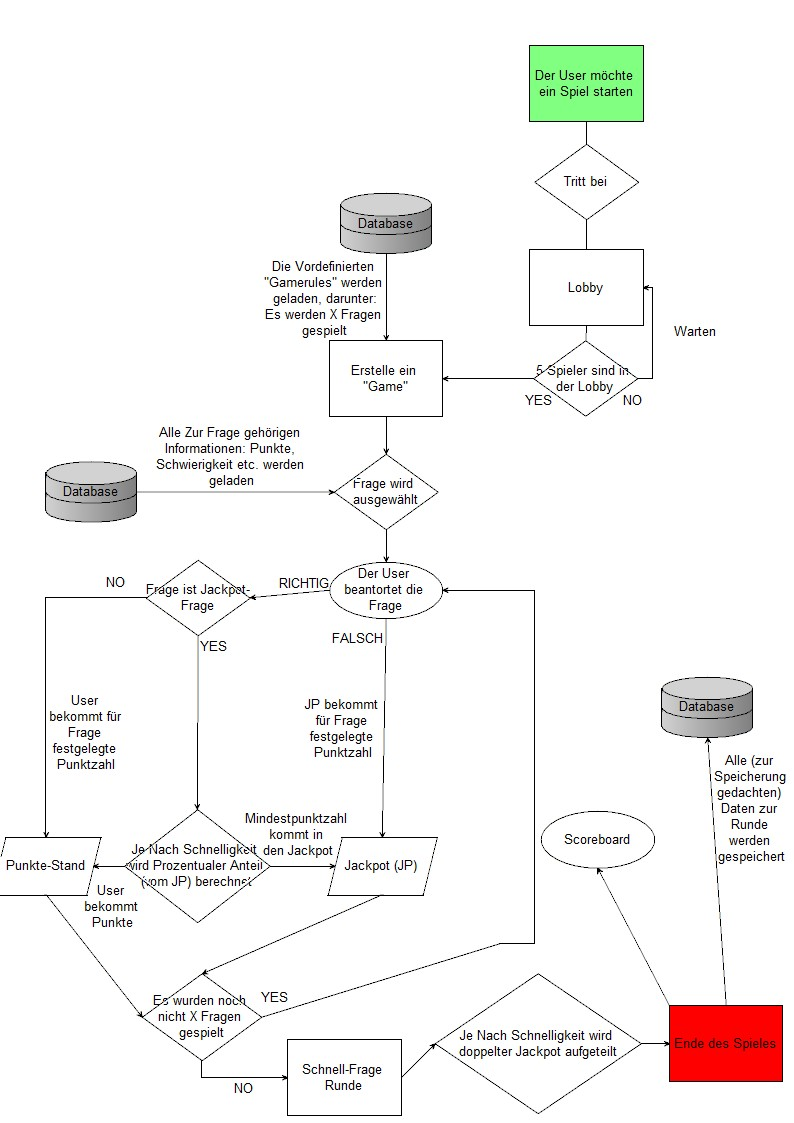
\includegraphics[width=0.9\textwidth, height=0.9\textheight]{Diagramm_002.jpg}
	\caption{Spielablauf als Diagramm}
	\label{img:Spielablauf}
\end{figure}
\subsection{Ablauf einer Spielrunde}
Der Spielablauf ist in der Grafik \ref{img:Spielablauf} auf Seite \pageref{img:Spielablauf} verdeutlicht.
Zm Anfang einer Spielrunde betritt ein Spieler die Lobby, in welcher er verweilt, bis mindestens fünf Spieler gefunden wurden. Ist dies geschehen, so beginnt das Spiel. Jeder Spieler der Gruppe erhält die gleiche Frage. Beantwortet er diese Frage korrekt, so erhält er die zu Frage zugehörige Punktzahl auf sein Konto, welches ihm stets angezeigt wird. Wird sie jedoch falsch beantwortet, so wandern die Punkte in einen Jackpot. Der Punktwert der Frage wird von ihrer Schwierigkeit beeinflusst (schwere Fragen bringen viele Punkte, leichtere Fragen dementsprechend weniger). Es kann durch Zufall eine Jackpot-Frage ausgelöst werden, in welcher um alle Punkte aus dem Jackpot gespielt wird. Die Jackpot-Frage ist von außen \textit{nicht} von den anderen Frage zu unterscheiden. Jeder, der die Jackpot-Frage richtig beantwortet, hat Garantie auf einen Anteil des Jackpots. Dieser Anteil wird anhand der Schnelligkeit der gegebenen (richtigen) Antwort bestimmt (Der Schnellste bekommt den größten Anteil, danach absteigend). Falls der Jackpot einmal leer ist (z.B. nach Jackpot-Frage) werden automatisch vom System eine gewisse Anzahl Punkte hineingegeben, um zu gewährleisten, dass stets Punkte im Jackpot sind, sollte z.B. die nächste Frage wieder eine Jackpot-Frage sein. Mit steigender Fragenanzahl (oder steigender Anzahl an falschen Antworten) erhöht sich die Wahrscheinlichkeit, dass eine Jackpot-Frage auftritt. Die letzte Frage einer Runde ist stets eine Jackpot-Frage. In dieser letzen Runde wird der Jackpot-Punktestand verdoppelt und um diesen gespielt. Als Option ist für die letzte Frage eine Schnellraterunde angedacht.
\subsection{An- und Abmelden}
\begin{description}
\item[/LF0010/] Registrierung \\
Ein Nutzer soll sich unter Angabe eines Nutzernamens, Passworts und E-Mail registrieren können.
\item[/LF0020/] Anmelden \\
Ein Nutzer soll sich mit seinem Nickname und Passwort einloggen können.
\item[/LF0030/] Abmelden \\
Der Nutzer soll sich vom System abmelden können.
\item[/LF0040/] Passwort anfordern \\
Der Nutzer soll sein Passwort anfordern können, wenn er dieses vergessen hat.
\item[/LF0050/] Spielerprofil \\
Für jeden Nutzer soll ein persönliches Profil existieren, dass mindestens den Name enthält
\end{description}
\subsection{Quiz}
\begin{description}
\item[/LF0060/] Fragenpool \\
Es muss ein Pool an Fragen zu einem Thema vorhanden ein, aus dem für das Quiz Fragen entnommen werden können.
\item[/LF0070/] Quizrunde \\
Jede Quizrunde soll dynamisch aus * Fragen zusammengestellt werden.
\item[/LF0080/] Antwort auswählen \\
Der Spieler soll aus * Antwortmöglichkeiten genau eine auswählen können, die richtig ist.
%LV: Die nächste Anforderung muss weitergehend spezifiziert werden bzw. um weitere Anforderungen erweitert werden, was einem zusätzlich noch angezeigt wird oder wann und wie sich ein Score verändert.
\item[/LF0090/]Auswertung einer Frage \\ 
Nach Auswahl einer Antwort soll die Anwendung eine Rückmeldung darüber geben, ob die richtige Antwort gewählt wurde. Falls nicht, so soll die richtige Antwort angezeigt werden %LV: Vielleicht auch, was die richtige Antwort war, wenn man falsch lag?
\item[/LF0100/] Ergebnisse ausgeben \\
Am Ende einer Quizrunde soll eine zusammenfassende Ausgabe der Ergebnisse erfolgen. Ergebnisse sind: Punktestand aller Teilnehmer (Scoreboard),  individuelle Platzierung.
\item[/LF0110/] Dauer einer Quizrunde \\
 Die Dauer einer Quizrunde ist intern, vom Administrator, einstellbar. Sie gilt dann für alle Spiele.
\end{description}
\subsection{Spielablauf einer Runde}
\begin{description}
\item[/LFXXXX/]gleiche Frage \\
 Jeder Spieler der Gruppe bekommt gleichzeitig die gleiche Frage bestellt.
\item[/LFXXXX/]Punkteausschüttung der Frage \\
Wird eine Frage richtig beantwortet, erhält der Spieler die zur Frage zugehörige Punktzahl auf sein Konto,  beantwortet er die Frage falsch, wandern die Punkte in einen Jackpot.
\item[/LFXXXX/]Jackpot-Frage \\
Eine Jackpot-Frage wird zufällig ausgelöst. Es wird um die Punkte im Jackpot gespielt. Äußerlich ist die Jackpot-Frage nicht von anderen Fragen zu unterscheiden.
\item[/LFXXXX/] Punkteausschüttung einer Jackpot-Frage \\
Jeder, der die Jackpot-Frage richtig beantwortet, erhält garantiert einen Anteil der Punkte. Dieser ist Abhängigkeit von der Schnelligkeit der gegebenen Antwort(der Schnellste bekommt am meisten, danach absteigend).
\item[/LFXXXX/] Auftrittswahrscheinlichkeit einer Jackpot-Frage \\
 Mit steigender Fragenanzahl (oder steigender Anzahl an falschen Antworten) wird die Wahrscheinlichkeit, dass eine Jackpot-Frage auftritt, höher.
\item[/LFXXXX/] Neufüllung des Jackpots nach Leerung \\
Wurde der Jackpot im Rahmen einer Jackpot-Frage ausgeschüttet, so wird automatisch vom System eine festgelegte Anzahl von Punkten in den Jackpot gegeben (Garantie, dass falls die nächste Frage wieder Jackpot-Frage ist, stets Punkte enthalten sind)
\item[/LFXXXX/]letzte Frage einer Spielrunde \\
Die letzte Frage einer Runde ist sicher eine Jackpot-Frage. Hierbei wird die Anzahl der Punkte im Jackpot verdoppelt und dann um diese gespielt.
\end{description}
\subsection{Speicherung der Daten}
\begin{description}
\item[/LF0130/] Speicherung von Fragen und Daten \\
Eine interne Datenbank verfügt über folgende Daten:
	\begin{itemize}
	\item Spielerbezogene Daten:
		\begin{itemize}
		\item Nutzername
		\item Login-Daten
		\item Spielerprofil
		\item Dashboard-Daten:
			\begin{itemize}
			\item durchschnittliche Antwortzeit
			\item Prozentsatz der richtigen Antworten
			\item durchschnittliche/höchste/gesamte Punktzahl
			\item insgesamt gespielte/gewonnen Runden
			\item Badges
			\end{itemize}
		\end{itemize}
	\item fragenbezogene Daten:
		\begin{itemize}
		\item Frage mit ID
		\item Antwortmöglichkeiten
		\item Schwierigkeit
		\item kann eine Jackpot-Frage sein?
		\item wie viele Punkte bringt die Frage
		\item[XXXX] Statistik, wie oft die Frage falsch/richtig beantwortet wurde
		\end{itemize}
	\end{itemize}
\end{description}
\subsection{Fragencharakteristiken}
\begin{description}
\item[/LFXXXX/] Schwierigkeitsgrad der Fragen \\
Jeder Frage wird initial in der Datenbank ein Schwierigkeitsgrad zugeordnet, welche vom Fragenersteller festgelegt wird. Werden bestimmte Fragen oft falsch beantwortet, so erhöht sich der Schwierigkeitsgrad dynamisch, wird sie oft richtig beantwortet, so wird der Schwierigkeitsgrad herabgesetzt.
\item[/LFXXXX/] Punktzahl einer Frage \\
Die Punktzahl einer Frage wird anhand des Schwierigkeitsgrades der Frage festgelegt. Ändert sich der Schwierigkeitsgrad, so muss auch die Punktzahl der Frage verändert werden.
\item[/LFXXXX/] Logik der Fragenauswahl \\
Generell erfolgt die Auswahl von Fragen, welche in einer Quizrunde gespielt werden, zufällig. Werden jedoch Fragen häufig falsch beantwortet, so ist die Wahrscheinlichkeit höher, dass diese Fragen öfter gespielt werden.
\item[/LF0140/] Import von Fragen \\
Es muss möglich sein, Fragen per Excel oder CSV in die Datenbank zu importieren.
\end{description}
\begin{description}
\item[/LF0150/] Access Control List \\
Folgende Kontrollzustände sollen eingerichtet werden:
	\begin{itemize}
	\item Administrator \\
	Dieser besitzt vollständige Zugriffsrechte und kann über eine externen Service Einstellungen verwalten, Fragen 				importieren und Rechte bearbeiten. Zusätzlich ist er in der Lage, Batches zu verwalten, also neue zu erstellen, zu 			bearbeiten und zu löschen
	\item User \\
	Dieser ist in der Lage, das Spiel zu spielen und seine persönlichen Daten einzusehen.
	\end{itemize}

\end{description}
%CS: denkt ihr wir sollten alle Gamification Elemente direkt als Muss-Ziel verankern? was wenn sich ergibt, dass es nicht/schlecht umsetzbar ist
\begin{description}
\item[/LF0160/] Badges \\
Für bestimmte Errungenschaften (bestimmte Punktzahl erreicht, besonders schnell geantwortet, besonders gute Statistiken) werden Abzeichen vergeben. Diese sind im System festgeschrieben und können nur durch den Administrator zentral bearbeiten/ verwaltet werden. Diese werden auf dem Dashboard ausgestellt und sofern der Benutzer es freigibt, auch auf dem Profil angezeigt.
\item[/LF0170/] Leaderboard \\
(siehe Spielmechaniken) Am Ende einer Runde soll eine Übersicht über Punktestände, Gewinner und (evtl.) Fragenübersicht angezeigt werden.
\end{description}
\subsection{Dashboard}
\begin{description}
\item[/LF0180/] Das persönliche Dashboard bildet eine Übersicht über folgende Daten: \\
	\begin{itemize}
	\item Fragenstatistiken:
		\begin{itemize}
		\item durchschnittliche Antwortzeit
		\item Prozentsatz der richtigen Antworten
		\item durchschnittliche/höchste/gesamte Punktzahl
		\item insgesamt gespielte/gewonnen Runden
		\end{itemize}
	\item Badges
	\item Anzahl bzw. Prozentsatz der erreichten freischaltbaren Inhalten
	\end{itemize}
\end{description}
\section{Kann-Ziele}
\subsection{Spielerprofil}
\begin{description}
\item[/LF0190/] optionale Profildetails \\ 
Für jeden Benutzer soll ein eigenes Profil anwählbar sein bestehend aus
	\begin{itemize}
	\item Nutzername
	\item Profilbild (optional)
	\item Kurze Nachricht (optional)
	\item Achievements
	\end{itemize}
\item[/LF0200/] Freischalten von Inhalten \\
Bestimmte Inhalte, wie z.B. andersfarbige Hintergründe, strategische Modifikatoren oder andere kosmetische Veränderungen (Verzierungen des Profils) sollen anhand der erspielten Punkte freigeschaltet werden.
\item[/LF0210/] Ratingsystem für Fragen \\
Es soll die Möglichkeit bestehen, nach Beantwortung einer Frage diese nach ihrer Qualität zu beurteilen.
\item[/LF0220/] optionale Ergebnisansicht am Ende einer Runde \\
Es soll weiterhin am Ende einer Runde möglich sein:
		\begin{itemize}
		\item eine Übersicht über alle Fragen mit den jeweils richtigen Antworten einzusehen,
		\item in dieser Runde erreichte Achievements anzuzeigen,
		\end{itemize}
\item[/LF0230/] Schnellfragerunde \\
Diese Runde ist die Letze einer Spielrunde und damit eine Jackpot-Frage.
Über eine bestimmte Zeitspanne können von jedem Spieler individuell so viele wie möglich Fragen beantwortet werden.
Je mehr Fragen richtig beantwortet wurden, desto mehr Anteile erhält man vom Jackpot.
\item[/LF0240/] Strategische Modifikatoren \\
Es können vor einer Spielrunde Modifikatoren ausgewählt werden, welche Vorteile und Nachteile besitzen. z.B.: doppelte Punktzahl gewinnbar, aber man verliert auch Punkte, etc.
\end{description}
\chapter{Nicht-funktionale Anforderungen}
\section{Muss-Ziele}
\subsection{Datenschutz und Anonymität}
\begin{description}
\item[/LL0250/] Profildetails \\
Der Spieler muss so wenig Details über sich bekanntgeben, wie er möchte. Minimal ist ein Benutzername festzulegen.
\item[/LL0260/] Bearbeitung des Profils \\ 
Der Nutzer kann sein Profil stets editieren, um Kontrolle über seine veröffentlichten Daten zu haben.
\item[/LL0270/] Löschung des Profils \\ 
Es muss für den User möglich sein, sein Profil zu löschen.
\end{description}
\section{Kann-Ziele}
\begin{description}
\item[/LL0280/]
\item[/LL0290/]
\item[/LL03XX/]
\end{description}

\chapter{Qualitätsmatrix nach ISO 25010}
% Erzeugt eine Tabelle. Die zweiten Parameter geben allgemeine Einstellungen für die Spalten an. l:linksbündig, c:center und r:rechtsbündig. Mit & wird eine Spalte erstellt, \\ erstellt eine neue Zeile. \hline erzeugt eine horizontale Linie.
\begin{tabular}{|l|c|c|c|c|}
\hline
		& hoch & mittel & niedrig& nicht anwendbar\\
\hline
Funktionalität  &x              &              & 		&\\     
Zuverlässigkeit	&              & x             & 		&\\
Effizienz 		&              &              & x		&\\
Sicherheit  	&              & x             & 		&\\
Kompatibilität  &              &x              & 		&\\
Benutzbarkeit  	& x             &              & 		&\\
Wartbarkeit  	&              &x              & 		&\\
Portierbarkeit  &              &x              & 		&\\
\hline
\end{tabular}

\chapter{Lieferumfang und Abnahmekriterium}
\begin{itemize}
\item Lieferumfang:
	\begin{itemize}
	\item Android-App als Client
	\item Server mit Datenbankanbindung
	\item Weboberfläche für den Administrator
	
	\end{itemize}
\item Abnahmekriterien:
	\begin{itemize}
	\item 
	\end{itemize}
\end{itemize}

\chapter{Vorprojekt}
\begin{itemize}
%CS: to discuss
\item Mögliches Vorprojekt: \\
Im Rahmen des Vorprojekts soll das wesentliche Grundgerüst, bestehend aus Datenbank, Server - und Client-Grundkonzept und Fragenmechanismus, erstellt werden. Dazu sollte es bereits möglich sein, Fragen in eine Datenbank mitsamt einer flexiblen Anzahl von Antwortmöglichkeiten einzulesen, zu speichern, sie abzufragen und anzeigen zu lassen. Es sollte weiterhin schon ein grundlegender Quizmechanismus implementiert werden, bei dem eine Frage mit mindestens vier Antwortmöglichkeiten gegeben ist und eine richtige Antwort enthält, welche der Spieler beantworten kann. Der Spieler muss weiterhin ein Feedback, in Form einer Nachricht o.ä., erhalten, um zu sehen, ob er die Frage richtig oder falsch beantwortet hat.
\end{itemize}

\chapter{Glossar}
\begin{description}
\item[E-Learning (Electronical Learning)]\ \\
Prozess des Lernens unter Beihilfe von elektronischen beziehungsweise von digitalen Medien.
\item[Gamification]\ \\
Ist der Einsatz von Spieltypischen Elementen und Vorgängen, die in einen spielfremden Zusammenhang gebracht werden. Ziel ist dabei die Motivationssteigerung des Anwenders für die Kernleistung. Häufig verwendete Spielmechaniken sind z.B. Punkte, Ziele und Errungenschaften.
%\item Feedback \\

\item[Quests]\ \\
Ist eine für den Benutzer formulierte Aufgabe, die in einer bestimmten Zeit zu absolvieren ist. Häufig werden sie in Verbindung mit anderen Aufgaben eingesetzt.
%\item[Achivements]\ \\

\item[Badges] \ \\
Bedeutet soviel wie "Abzeichen". Sie repräsentieren das Vorhandensein bestimmter Fertigkeiten, Fähigkeiten oder Kenntnisse in bestimmten Bereichen oder als Beleg für die Teilnahme an bestimmten Veranstaltungen. Badges sind eine Form von Feedback.
\item[ACL (Access Control List)]\ \\
Technik zur Vergabe von Zugriffsrechten, z.B. für Nutzer und Anwendungen. Es ist eine feine Unterteilung in verschiedene Zugriffsgruppen möglich.
\end{description}
\end{document}